% This is file JFM2esam.tex
% first release v1.0, 20th October 1996
%       release v1.01, 29th October 1996
%       release v1.1, 25th June 1997
%       release v2.0, 27th July 2004
%       release v3.0, 16th July 2014
%   (based on JFMsampl.tex v1.3 for LaTeX2.09)
% Copyright (C) 1996, 1997, 2014 Cambridge University Press

\documentclass{jfm}
\usepackage{graphicx}
%\usepackage{epstopdf, epsfig}
\usepackage{physics}

\usepackage{enumitem,amssymb}
\newlist{todolist}{itemize}{2}
\setlist[todolist]{label=$\square$}
\usepackage{pifont}
\newcommand{\cmark}{\ding{51}}%
\newcommand{\xmark}{\ding{55}}%
\newcommand{\done}{\rlap{$\square$}{\raisebox{2pt}{\large\hspace{1pt}\cmark}}%
\hspace{-2.5pt}}
\newcommand{\wontfix}{\rlap{$\square$}{\large\hspace{1pt}\xmark}}

\newtheorem{lemma}{Lemma}
\newtheorem{corollary}{Corollary}

\newcommand{\cz}{c_{\zeta}}
\newcommand{\cs}{c_{\psi}}
\newcommand{\ct}{c_{\theta}}
\newcommand{\cu}{c_u}
\newcommand{\css}{c_{\psi \psi}}
\newcommand{\csz}{c_{\psi \zeta}}
\newcommand{\czs}{c_{\zeta \psi}}
\newcommand{\czz}{c_{\zeta \zeta}}
\newcommand{\ctz}{c_{\theta \zeta}}
\newcommand{\czt}{c_{\zeta \theta}}
\newcommand{\ctt}{c_{\theta \theta}}
\newcommand{\cst}{c_{\psi \theta}}
\newcommand{\cts}{c_{\theta \psi}}
\newcommand{\Rayleigh}{\mbox{\textit{Ra}}}  % Rayleigh number
\newcommand{\Pra}{\mbox{\textit{Pr}}}  % Prandtl number


\shorttitle{CE2 Busse Annulus}
\shortauthor{J. S. Oishi, K. J. Burns, J. B. Marston, S. M. Tobias}

\title{Direct Statistical Simulation of the Busse Annulus}

\author{Jeffrey S. Oishi\aff{1}
  \corresp{\email{joishi@bates.edu}},
  Keaton J. Burns\aff{2,3},
  J. B. Marston\aff{4},
 \and Steven M. Tobias\aff{5}}

\affiliation{\aff{1}Department of Physics \& Astronomy, Bates College,
Lewiston, ME 04240, USA
\aff{2} Department of Mathematics, Massachusetts Institute of Technology, Cambridge, MA 02138 USA
\aff{3} Center for Computational Astrophysics, Flatiron Institute, New York, NY 10010, USA
\aff{4} Department of Physics, Brown University, Providence, RI 02912, USA
\aff{5} Department of Applied Mathematics, University of Leeds, Leeds LS2 9JT, UK
}

\begin{document}

\maketitle

\begin{abstract}
We consider direct statistical simulation (DSS) of a paradigm system of convection interacting with mean flows. In the Busse Annulus model zonal jets are generated through the interaction of convectively driven turbulence and rotation; non-trivial dynamics including the emergence of multiple jets and bursting 'predator-prey' type dynamics can be found. We formulate the DSS by expanding around the mean flow in terms of equal-time cumulants and arrive at a closed set of equations of motion for the cumulants. Here, we present results using an expansion terminated at the second cumulant (CE2); it is fundamentally a quasi-linear theory.
We focus on a particular cases including bursting and bistable multiple jets and demonstrate that CE2 can reproduce the results of direct numerical simulation if particular attention is given to symmetry considerations. 
%in which the direct numerical simulation yields an initial three-jet solution that is unstable to a two-jet solution.
%Interestingly, CE2 predicts a stable three-jet solution, though we find that by biasing the initial conditions to favor certain symmetries, CE2 reproduces the DNS results.
\end{abstract}

\begin{keywords}
\end{keywords}

\section{Introduction}
\label{sec:intro}

Moved from abstract: Turbulent systems generate and interact with mean flows in a wide variety of natural systems.
Understanding the nature of these interactions, particularly for systems far from equilibrium, remains a key problem for the description of large-scale flows on planets and stars.
The fundamental problem in studying such systems via direct numerical simulation (DNS) is the expense of the calculations owing to the vast range of spatial and temporal scales that need to be described. 
One way to make progress is to study the statistics of the flow rather than detailed flow variables themselves. However, these systems are often inhomogeneous and strongly anisotropic, and such a statistical description should respect this.

Rotation is a hallmark of geophysical and astrophysical fluid dynamics.
Through the breaking of reflectional symmetry, rotating systems are known to generate mean flows such as zonal jets; examples of which include the bands on Jupiter, the jet stream on Earth and the differential rotation in stars.
It is common that the production of these jets is driven by rotating convection.

%Understanding the interaction between turbulence and mean flows remains a major challenge as such systems are often at extreme parameters inaccessible to direct numerical simulation (DNS).

Here, we explore one particular system, the Busse Annulus, using the CE2 formulation of direct statistical simulation.
CE2 is a cumulant expansion truncated at second order and is fundamentally quasilinear.
Our recent work \citep{2018RSPSA.47480422T} has shown that in direct simulation, the generalized quasilinear approximation (GQL) outperforms QL models at all parameter values explored.

The Busse annulus model considers convection in a duct with slanted ends leading to a topographic $\beta$ effect.
This system present an important challenge for CE2, as it is possesses a linear instability which is known to host multiple solutions at modest Rayleigh numbers \citep{bh1993}.
How does a quasilinear statistical theory fare when faced with multiple potential solution basins?
In particular, we investigate the sensitivity of CE2 to initial conditions for a case with multiple solution branches.

\section{Model Equations, Formulation, Parity and Numerical Methods}
\label{sec:model-eqations}

We consider the equations for the Busse annulus \citep[see e.g.][]{bh1993} in a Cartesian system $(x,y,z)$ and write the two-dimensional equation of motion in terms of the $z$-component of the vorticity, $\zeta = \laplacian{\psi}$ as
\begin{equation}
  \label{eq:zeta_eom}
  \pdv{\zeta}{t} + J(\psi, \zeta) - \beta \pdv{\psi}{x} = -\frac{\Rayleigh}{\Pran} \pdv{\theta}{x} -C |\beta|^{1/2} \zeta + \laplacian{\zeta}
\end{equation}
where $\psi$ is the streamfunction and $(u,v) = (-\pdv*{\psi}{y}, \pdv*{\psi}{x})$ is defined by
\begin{equation}
  \label{eq:zeta_def}
  \zeta = \laplacian{\psi},
\end{equation}
Here the jacobian $J(A, B) = \pdv*{A}{x}\pdv*{B}{y} - \pdv*{A}{y}\pdv*{B}{x}$ is the Jacobian. 
The temperature pertubation from a linear basic state is given by $\theta$, where
%
\begin{equation}
  \label{eq:theta}
  \pdv{\theta}{t} + J(\psi, \theta) = -\pdv{\psi}{x} + \frac{1}{\Pran} \nabla^2 \theta.
\end{equation}
The system is thus governed by four dimensionless parameters, $\beta$, $C$, $\Pran = \nu/
\kappa$, and $\Rayleigh = \alpha g \Delta T d^3/\nu \kappa$ \citep[see e.g.][]{rj2006}

DSS at CE2 is implemented by first defining the averaging procedure to be a zonal average, e.g. $\langle f(x,y) \rangle = 1/L_x \, \int_0^{L_x} f(x,y) \, dx$ and deriving evolution equations we need equations for the first cumulants $\cz(y) = \langle \zeta \rangle $ and $\ct(y) = \langle \theta \rangle$, and the second cumulants 
\begin{equation}
    \ctt(\xi,y_1,y_2) = \langle \zeta^\prime(x_1,y_1) \zeta^\prime(x_2,y_2) \rangle
\end{equation}
and $\xi = x_1 - x_2$; similar definitions are used for the second cumulants $\czz$, $\ctz$, and $\czt$. 
Cumulants involving $\psi$ and $\zeta$ are related by differential operators \citep[see e.g.][]{2013PhRvL.110j4502T}.
Because the equations require both $\psi$ and $\zeta$ cumulants, we solve for $\cs$, $\ct$, $\css$, $\cts$, $\cst$, and $\ctt$, though we write equations in terms of $\zeta$ cumulants.

We solve dynamical equations for the cumulants,
\begin{equation}
  \label{eq:cz}
  \pdv{\cz}{t} = - \qty(\pdv{y_1} + \pdv{y_2}) \pdv{\csz}{\xi}\eval_{\xi \to 0}^{y_1 \to y_2} - C |\beta|^{1/2} \cz + \pdv[2]{\cz}{y_1},
\end{equation}

\begin{equation}
  \label{eq:czz}
  \begin{split}
    \pdv{\czz}{t} &= \pdv{\cs}{y_1} \pdv{\czz}{\xi} - \qty(\pdv{\cz}{y_1} - \beta) \pdv{\csz}{\xi} - \pdv{\cs}{y_2} \pdv{\czz}{\xi}  + \qty(\pdv{\cz}{y_2} - \beta) \pdv{\czs}{\xi}\\
    &+ \frac{\Rayleigh}{\Pran} \qty(\pdv{\czt}{\xi} -  \pdv{\ctz}{\xi}) - 2C |\beta|^{1/2} \czz + (\nabla_1^2 + \nabla_2^2) \czz,    
  \end{split}
\end{equation}

\begin{equation}
  \label{eq:ct}
  \pdv{\ct}{t} = - \qty(\pdv{y_1} + \pdv{y_2}) \pdv{\cst}{\xi} \eval_{\xi \to 0}^{y_1 \to y_2} + \frac{1}{\Pran} \pdv[2]{\ct}{y_1}l,
\end{equation}

\begin{equation}
  \label{eq:ctt}
\begin{split}
  \pdv{\ctt}{t} &= \pdv{\cts}{\xi} - \pdv{\cst}{\xi} + \left(\pdv{\cs}{y_1} - \pdv{\cs}{y_2}\right)\pdv{\ctt}{\xi} + \pdv{\ct}{y_2}\pdv{\cts}{\xi} - \pdv{\ct}{y_1}\pdv{\cst}{\xi}\\
&  + \frac{1}{\Pran}(\nabla_1^2 + \nabla_2^2) \ctt
\end{split}
\end{equation}

\begin{equation}
  \label{eq:ctz}
  \begin{split}
    \pdv{\ctz}{t} &= \qty(\pdv{\cs}{y_1} - \pdv{\cs}{y_2}) \pdv{\ctz}{\xi} - \qty(1 + \pdv{\ct}{y_1}) \pdv{\csz}{\xi} + \qty(\pdv{\cz}{y_2} - \beta) \pdv{\cts}{\xi}\\
    &  - C |\beta|^{1/2} \ctz + \frac{1}{\Pran} \nabla_1^2 \ctz + \nabla_2^2 \ctz.
  \end{split}
\end{equation}
Other second cumulant terms can be calculated from symmetry considerations.
% This could be calculated using symmetry, $\czt(y_1, y_2, \xi) = \ctz(y_2, y_1, -\xi)$.
% However, because we use IMEX timestepping and such symmetry operations can only be applied at the end of a timestep, this would mean that $\czt$ would not be updated during the implicit step.
% Instead, we solve an equation for $\czt$ which is identical to equation~(\ref{eq:ctz}) with $x_1,y_1$ and $x_2, y_2$ swapped.


%\subsection{Parity}
%\label{sec:parity}

We solve the system subject to impenetrable, stress-free boundary conditions in the $y$ dimension; it is periodic in $x$. 
This means that $\theta$, $\zeta$, and $\psi$ all have odd parity.
The action of the zonal average preserves the parity, and so we discretize the first cumulants $\cz$, $\ct$ using a $\sin$ series. 

%\subsection{Numerical Methods}
%\label{sec:numerical}

We use \emph{Dedalus} \citep{2020PhRvR...2b3068B} to solve both the direct equations (\ref{eq:zeta_eom} - \ref{eq:theta}) and the CE2 model equations, (\ref{eq:cz})-~(\ref{eq:ctz}).
For the CE2 equations, we use explicit timestepping for all variables.
We have found this to be more stable than the typical approach of using implicit-explicit (IMEX) timesteppers in which the linear terms are implicitly advanced while the explicit terms explicit.
The DNS results do, however, use IMEX schemes in the manner typical for Dedalus.


\section{Results}
\label{sec:results}

We begin each CE2 simulation using one of two extreme initial conditions: \emph{maximum ignorance}, in which we assume a completely uncorrelated $\ctt$ and all other fields zero, and \emph{maximum knowledge}, in which we initialize all fields using cumulants calculated from a DNS solution. This allows us to evaluate CE2's ability to both \emph{find} solutions and \emph{continue} solutions already known.

In order to facilitate comparison with previous work, we adapt the same run naming scheme as in \citet{2018RSPSA.47480422T}.

\begin{table}
  \begin{center}
\def~{\hphantom{0}}
  \begin{tabular}{lcccccl}
    Run & $\beta$ & $\Rayleigh$ & $C$ & DNS Resolution & CE2 Resolution & Comment \\[3pt]
    A  & $2.8\times 10^3$ & $7.6 \times 10^4$   & $0$ & $256 \times 64$ & $32^3$ & Two-jet \\
    B  & $7.07\times 10^5$ & $10^8$ & $0.316$ & $512 \times 256$ & $128 \times 64$ & Seven-jet  \\
    C  & $5\times 10^5$ & $8\times 10^7$ & $0$ & $512 \times 256$ & $256 \times 64$ & three-jet $\to$ two-jet bursting \\
    R  & $3.16\times 10^5$ & $4\times 10^7$ & $0.316$ & $256 \times 64$ & $128\times 64^2$ & Five-jet\\
  \end{tabular}
  \caption{Runs}
  \label{tab:runs}
  \end{center}
\end{table}

\subsection{Run A: 2 Jet/3 Jet solutions}
\label{sec:hov}

We begin by comparing the time evolution of the zonal average jets, $\left< u \right>(y, t)$ in DNS and CE2 simulations.

Figure~\ref{fig:run_A} shows the time evolution of run A: for random initial conditions, the DNS solution selects a seemingly stable 2-jet solution.
CE2, on the other hand finds a 3-jet solution.
At these parameters, however, there are both 2-jet and 3-jet solutions known: the 3-jet solutions are unstable to perturbations that break shift-reflect symmetry \citep{bh1993}. Using Dedalus, we ran a DNS with initial conditions that respect this symmetry. Owing to our highly accurate spectral methods, the 
\begin{figure}
  \centering
  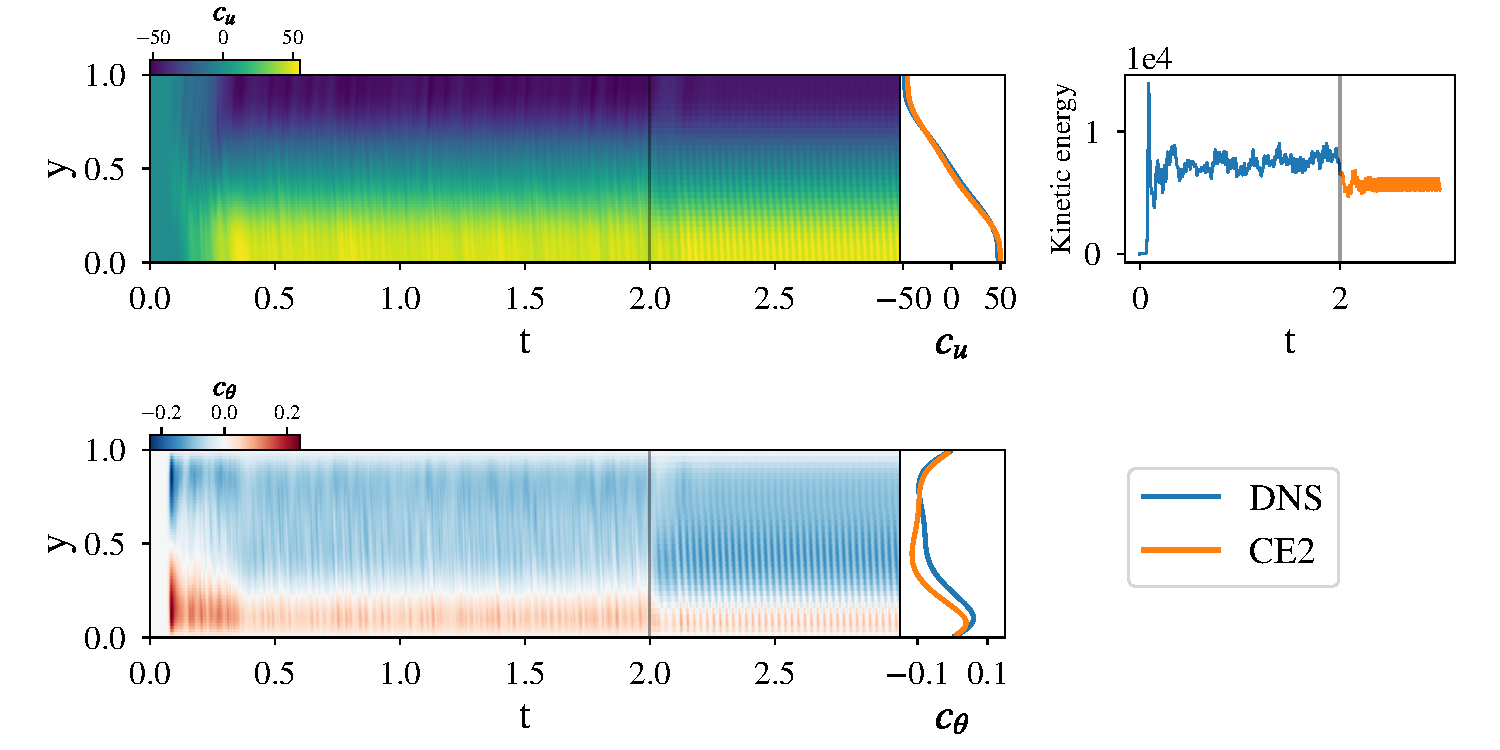
\includegraphics[width=\textwidth]{../../figs/run_A_fig.pdf}
  \caption{Left: hovmoller diagrams of first cumulants $\cu$ (upper), $c_\theta$ (lower) from run A started in DNS and continued at $t=2$ with DNS. Middle: time-averaged first cumulants as a function of $y$ for both CE2 and DNS averaged over $1 \le t \le 2$ for DNS and $2 \le t \le 3$ for CE2. Right: total kinetic energy.}
  \label{fig:run_A}
\end{figure}

\begin{figure}
  \centering
  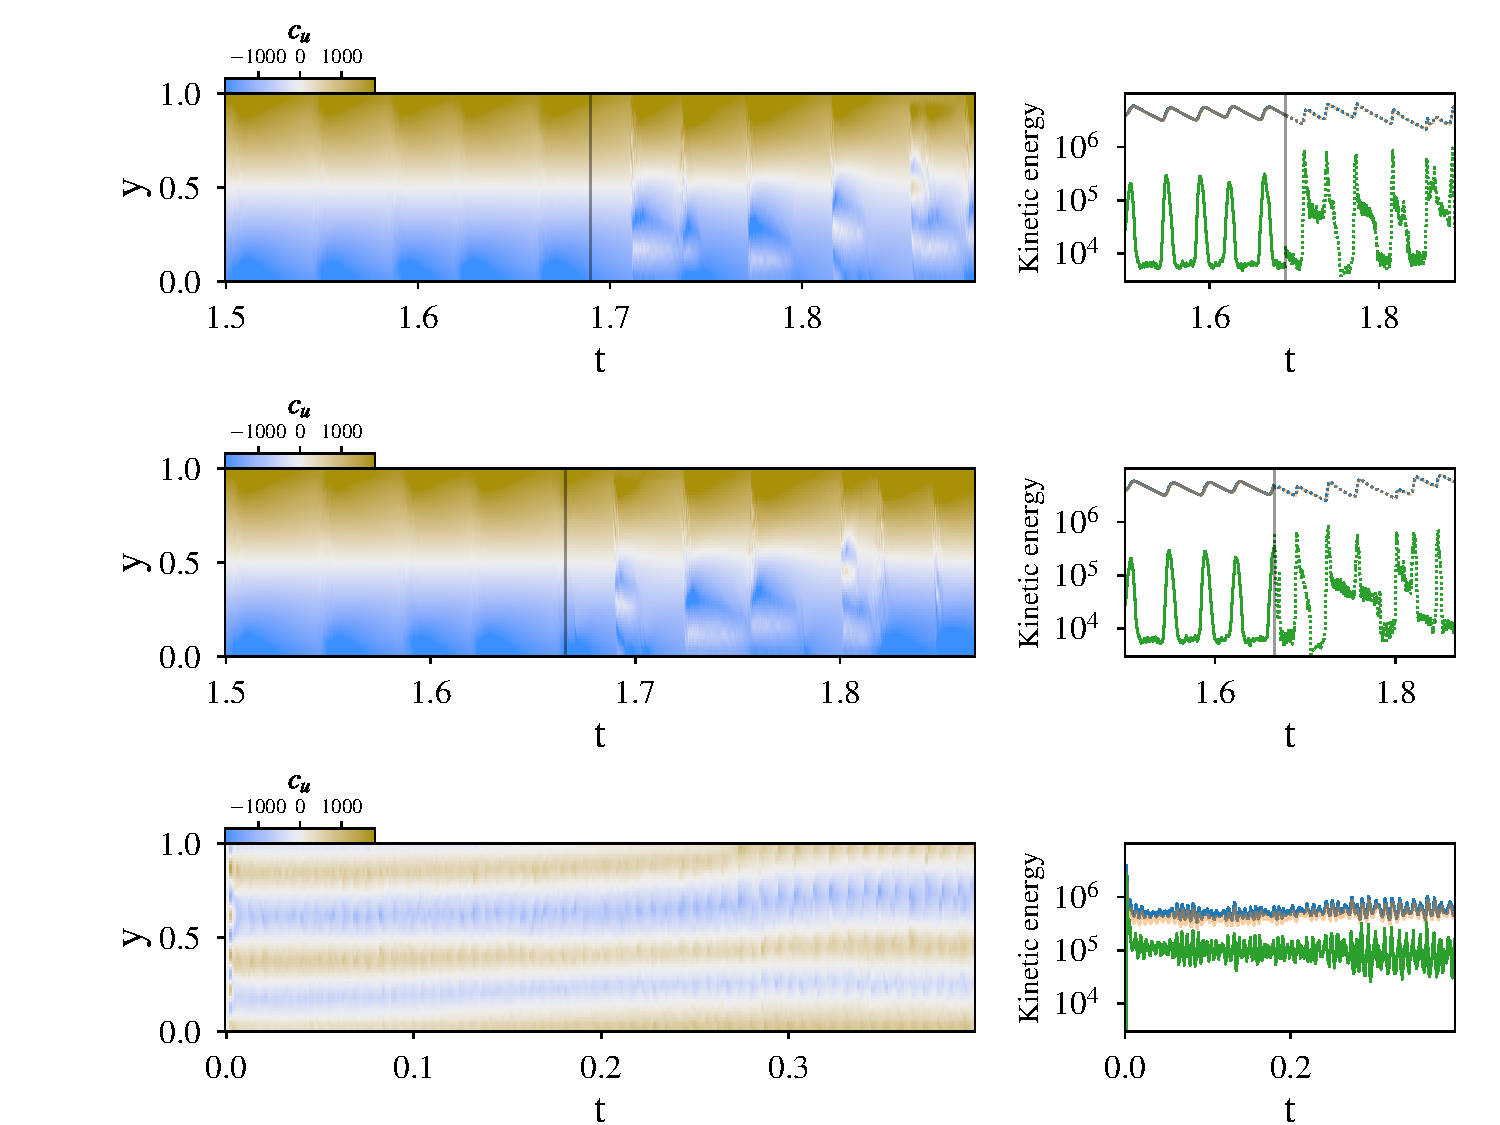
\includegraphics[width=\textwidth]{../../figs/run_C_fig.pdf}
  \caption{Run C Hovmuller diagrams of $\cu$ (left) and total, zonal, and non-zonal kinetic energies (right). Solid lines are DNS; dotted lines are CE2. From top to bottom: ``Maximum knowledge'' CE2 run started from quiescent state of DNS solution, ``maximum knowledge'' started from bursting state of DNS solution, ``maximum ignorance'' CE2 initialized from a diagonal $\ctt$. Within each row, left to right: hovmoller diagram. }
  \label{fig:run_C}
\end{figure}

\begin{figure}
    \centering
    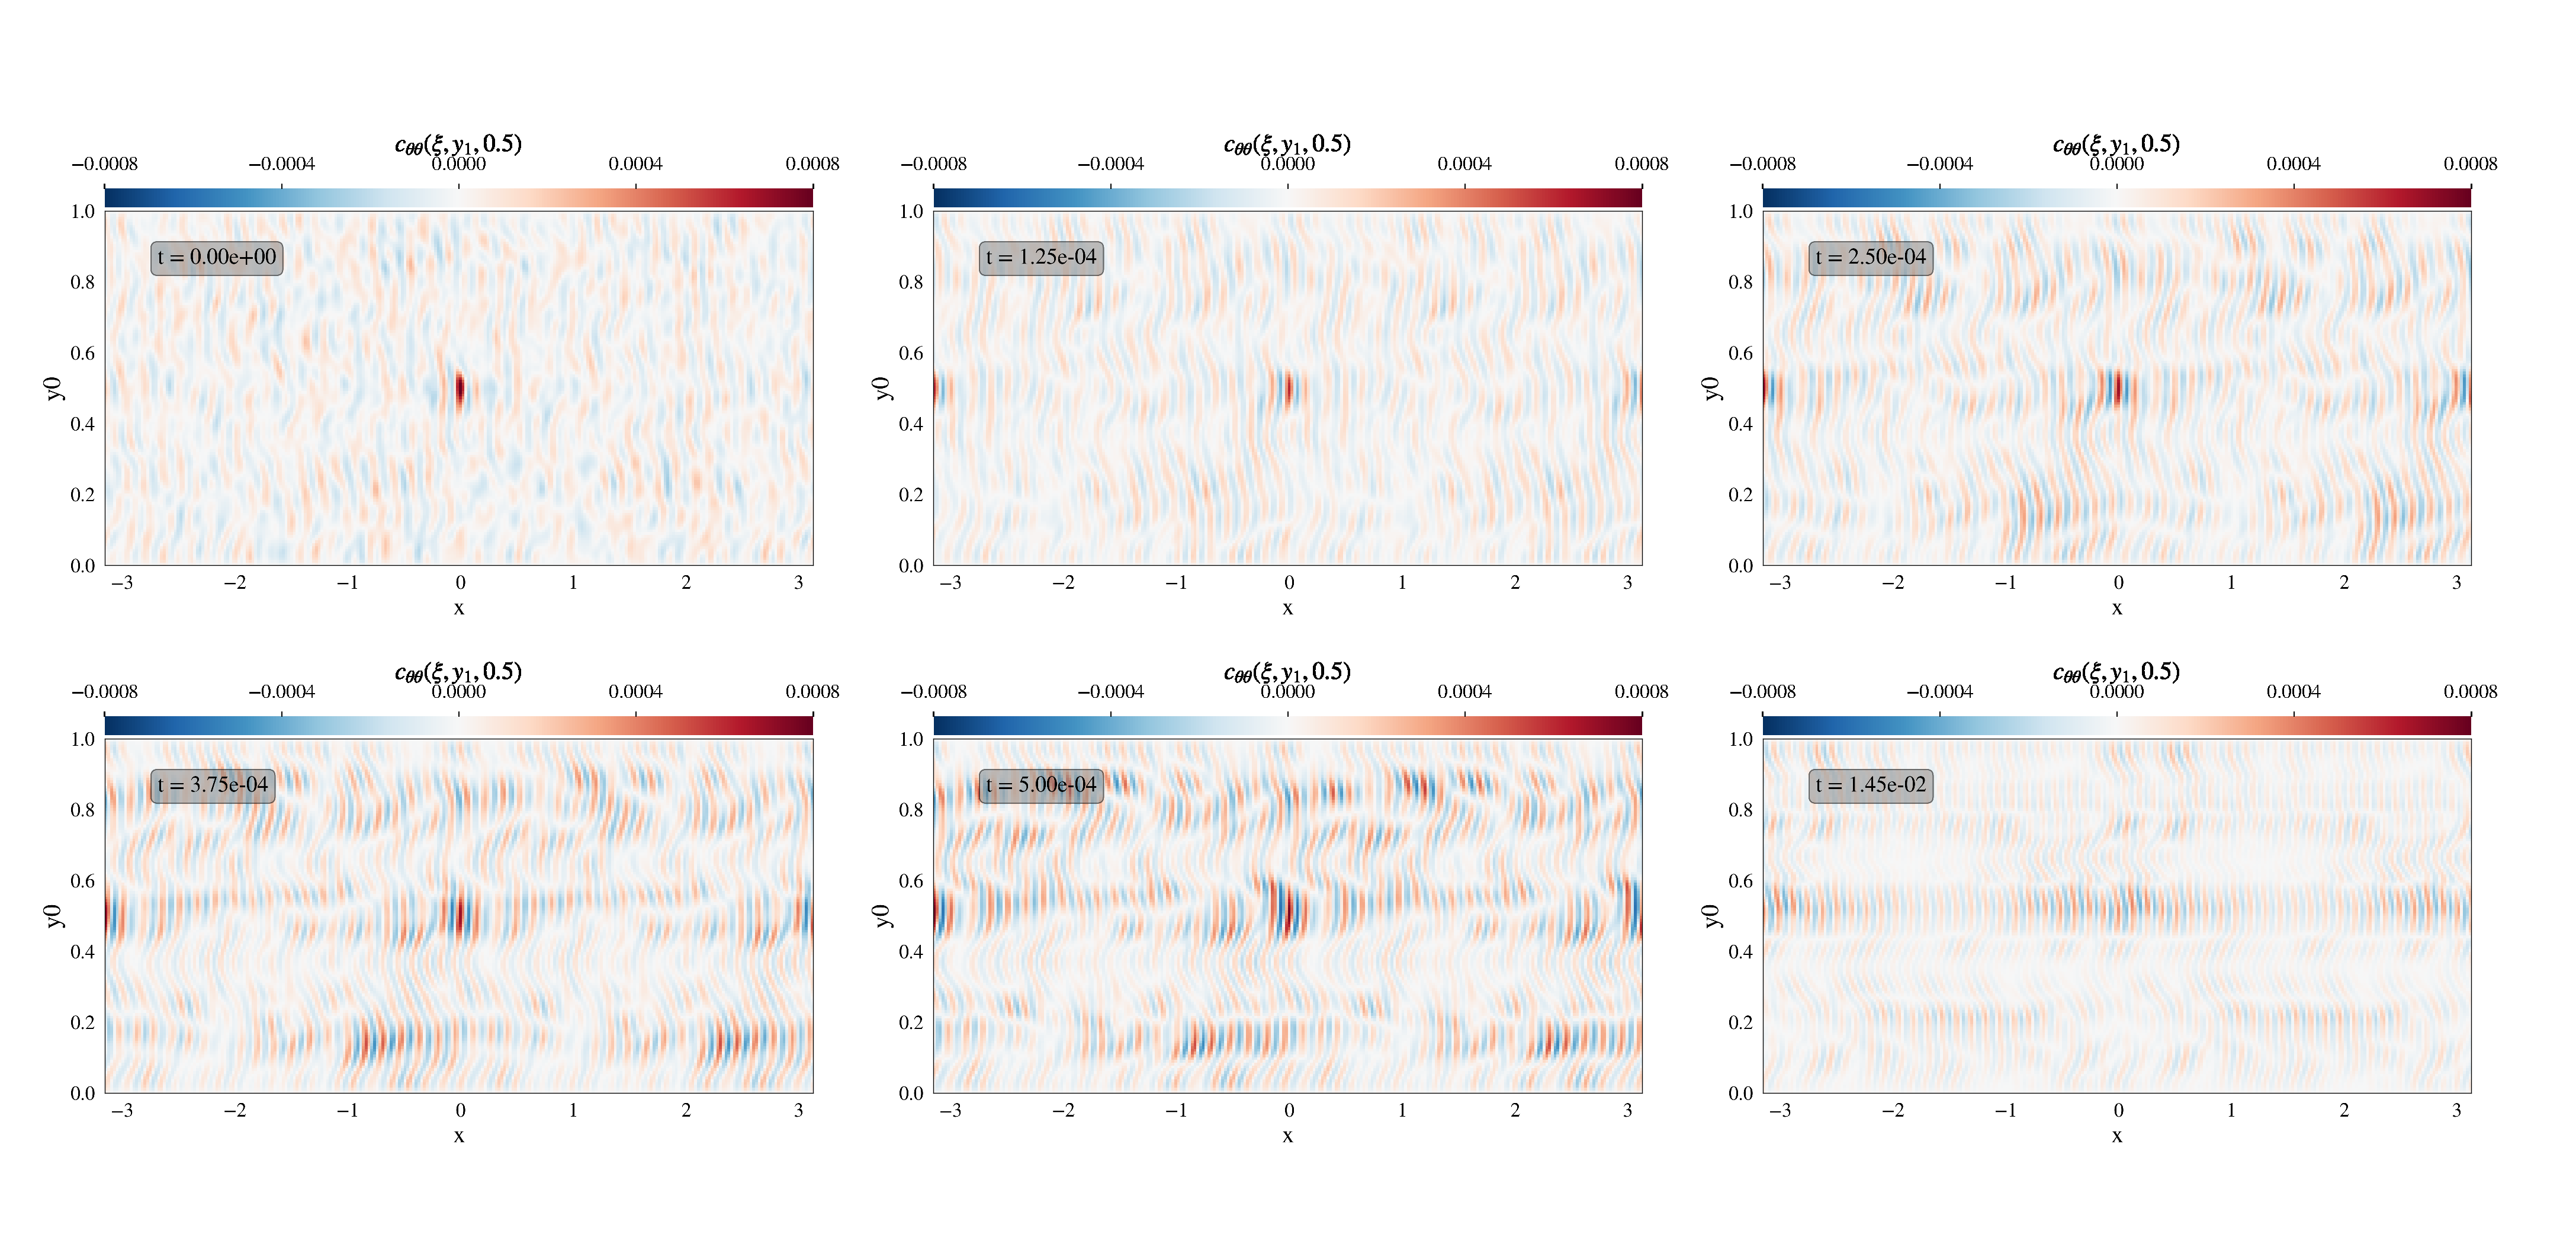
\includegraphics[width=\textwidth]{../../figs/run_B_decoherence.pdf}
    \caption{$\ctt(\xi, y_1, y_2 = 0.5)$ as a function of time for run B with ``maximum knowledge'' initial conditions selected from the output of DNS. Note that the initial, tightly peaked $\ctt$ from DNS (left most panel) quickly delocalizes and reverts to the overemphasis of long-range correlations characteristic of CE2.}
    \label{fig:run_B_decoherence}
\end{figure}
At higher $\Rayleigh$, run R shows 
\begin{figure}
  \centering
  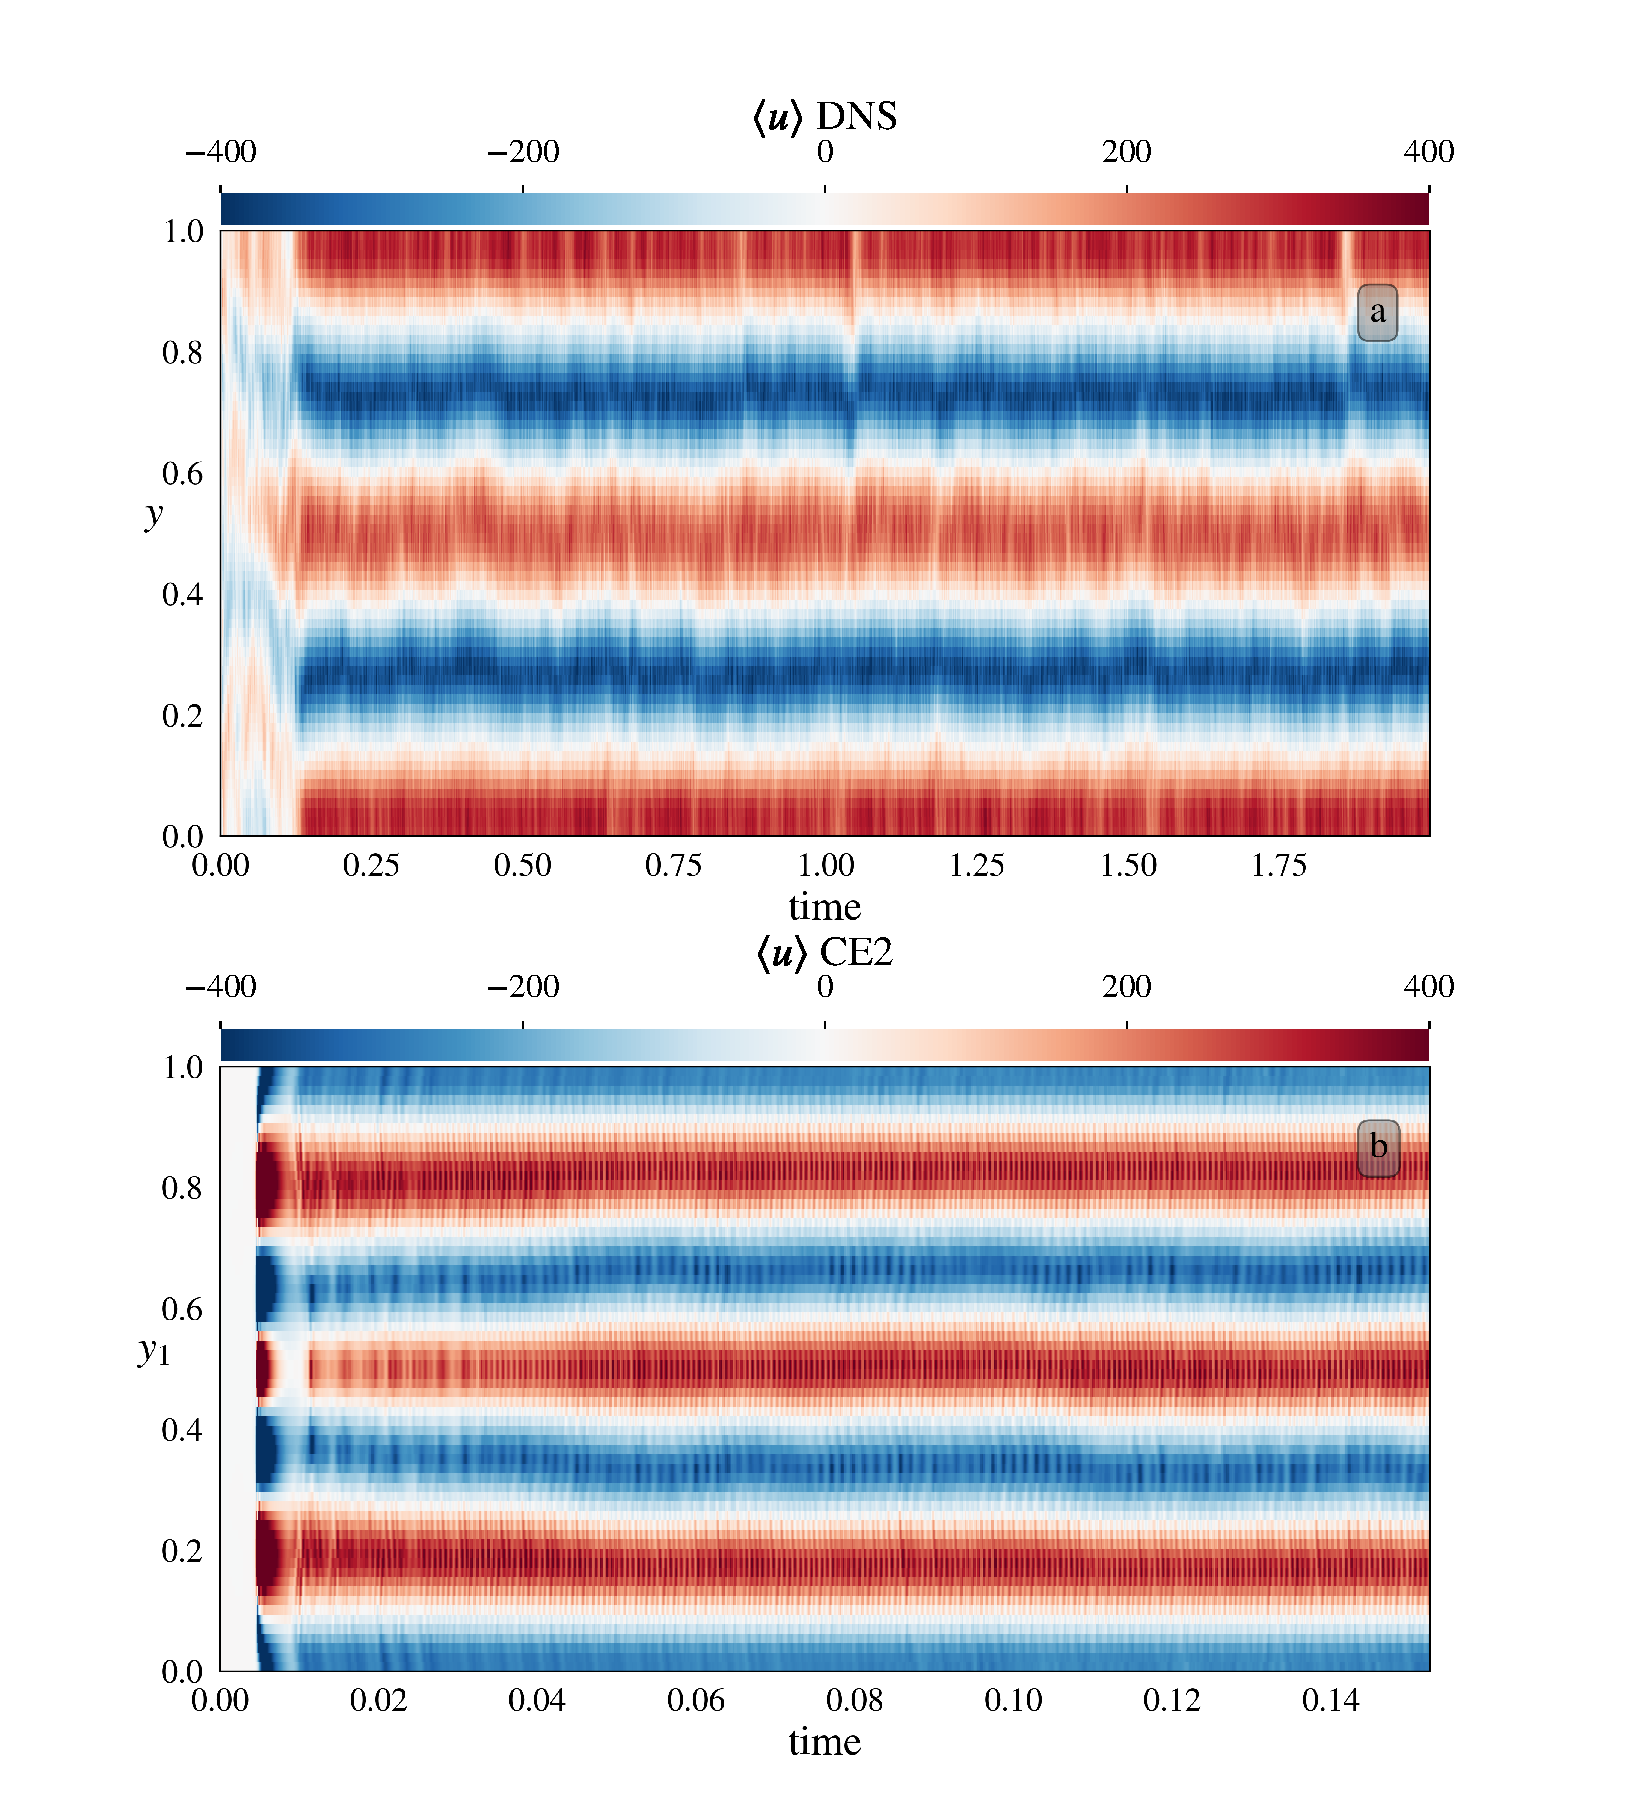
\includegraphics[width=0.5\textwidth]{../../figs/hov_cu_dns_ce2_run_R.pdf}
  \caption{Hovmoller diagram of run R in both DNS (a) and CE2 (b). The first cumulant $\cu$ is zero at $t = 0$. CE2 picks up a stable 7-jet solution.}
  \label{fig:hov_run_R}
\end{figure}
\begin{figure}
  \centering
  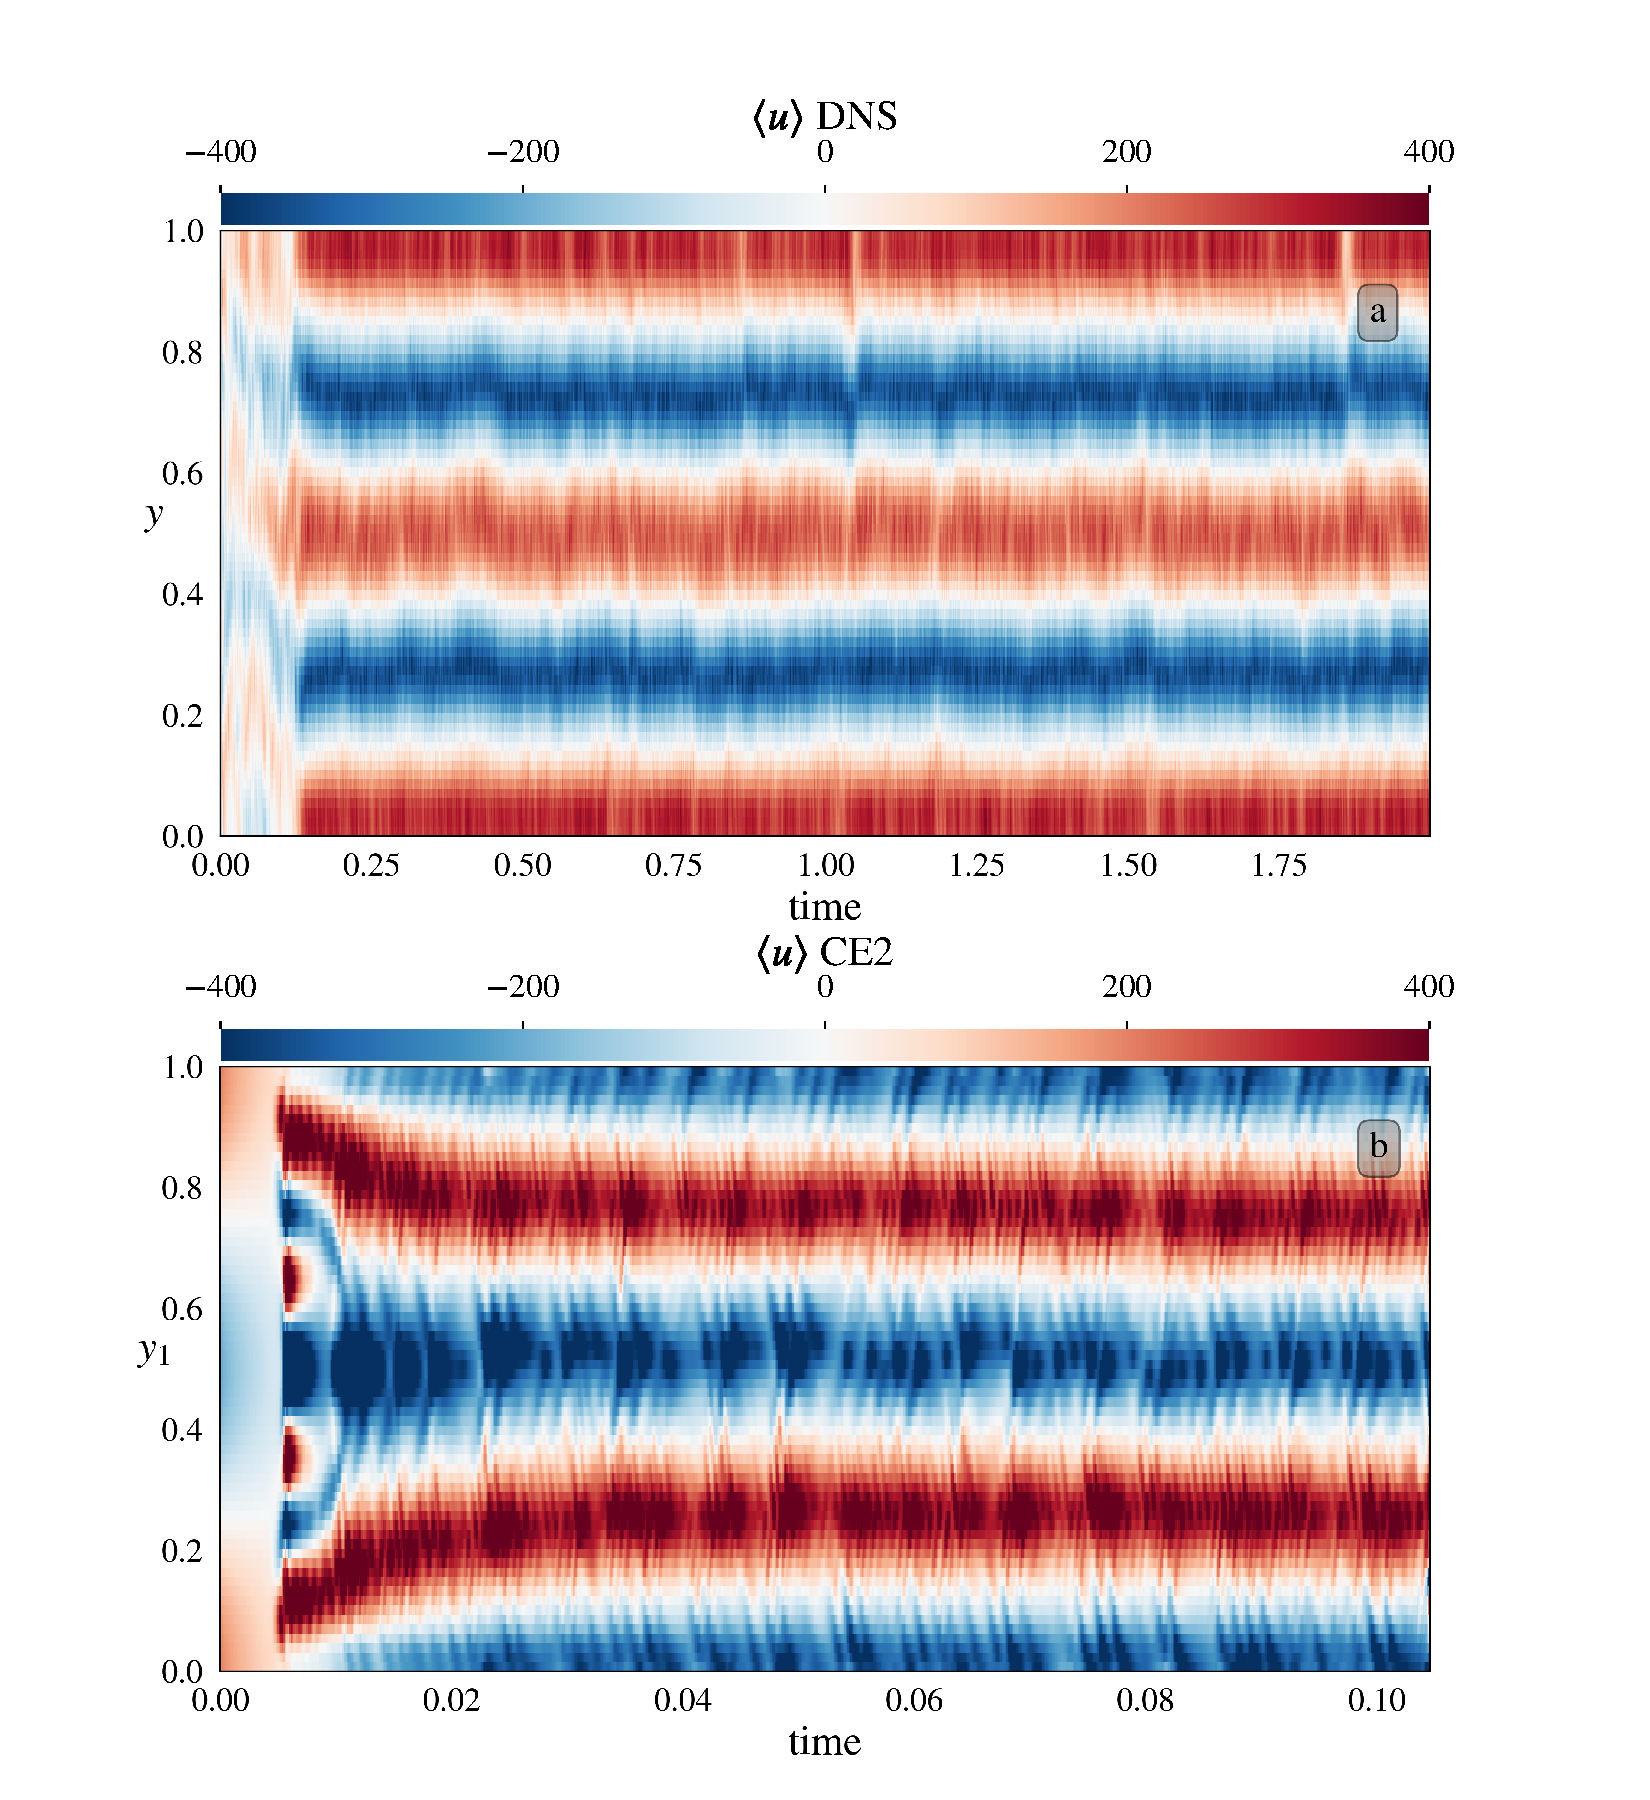
\includegraphics[width=0.5\textwidth]{../../figs/hov_cu_dns_ce2_run_S.pdf}
  \caption{Hovmoller diagram of run R in both DNS (a) and CE2 (b) with the CE2 solution biased with a 3-jet solution at $t=0$. In this case, CE2 latches on to the correct 5-jet solution.}
   \label{fig:hov_run_S}
\end{figure}
\begin{figure}
  \centering
  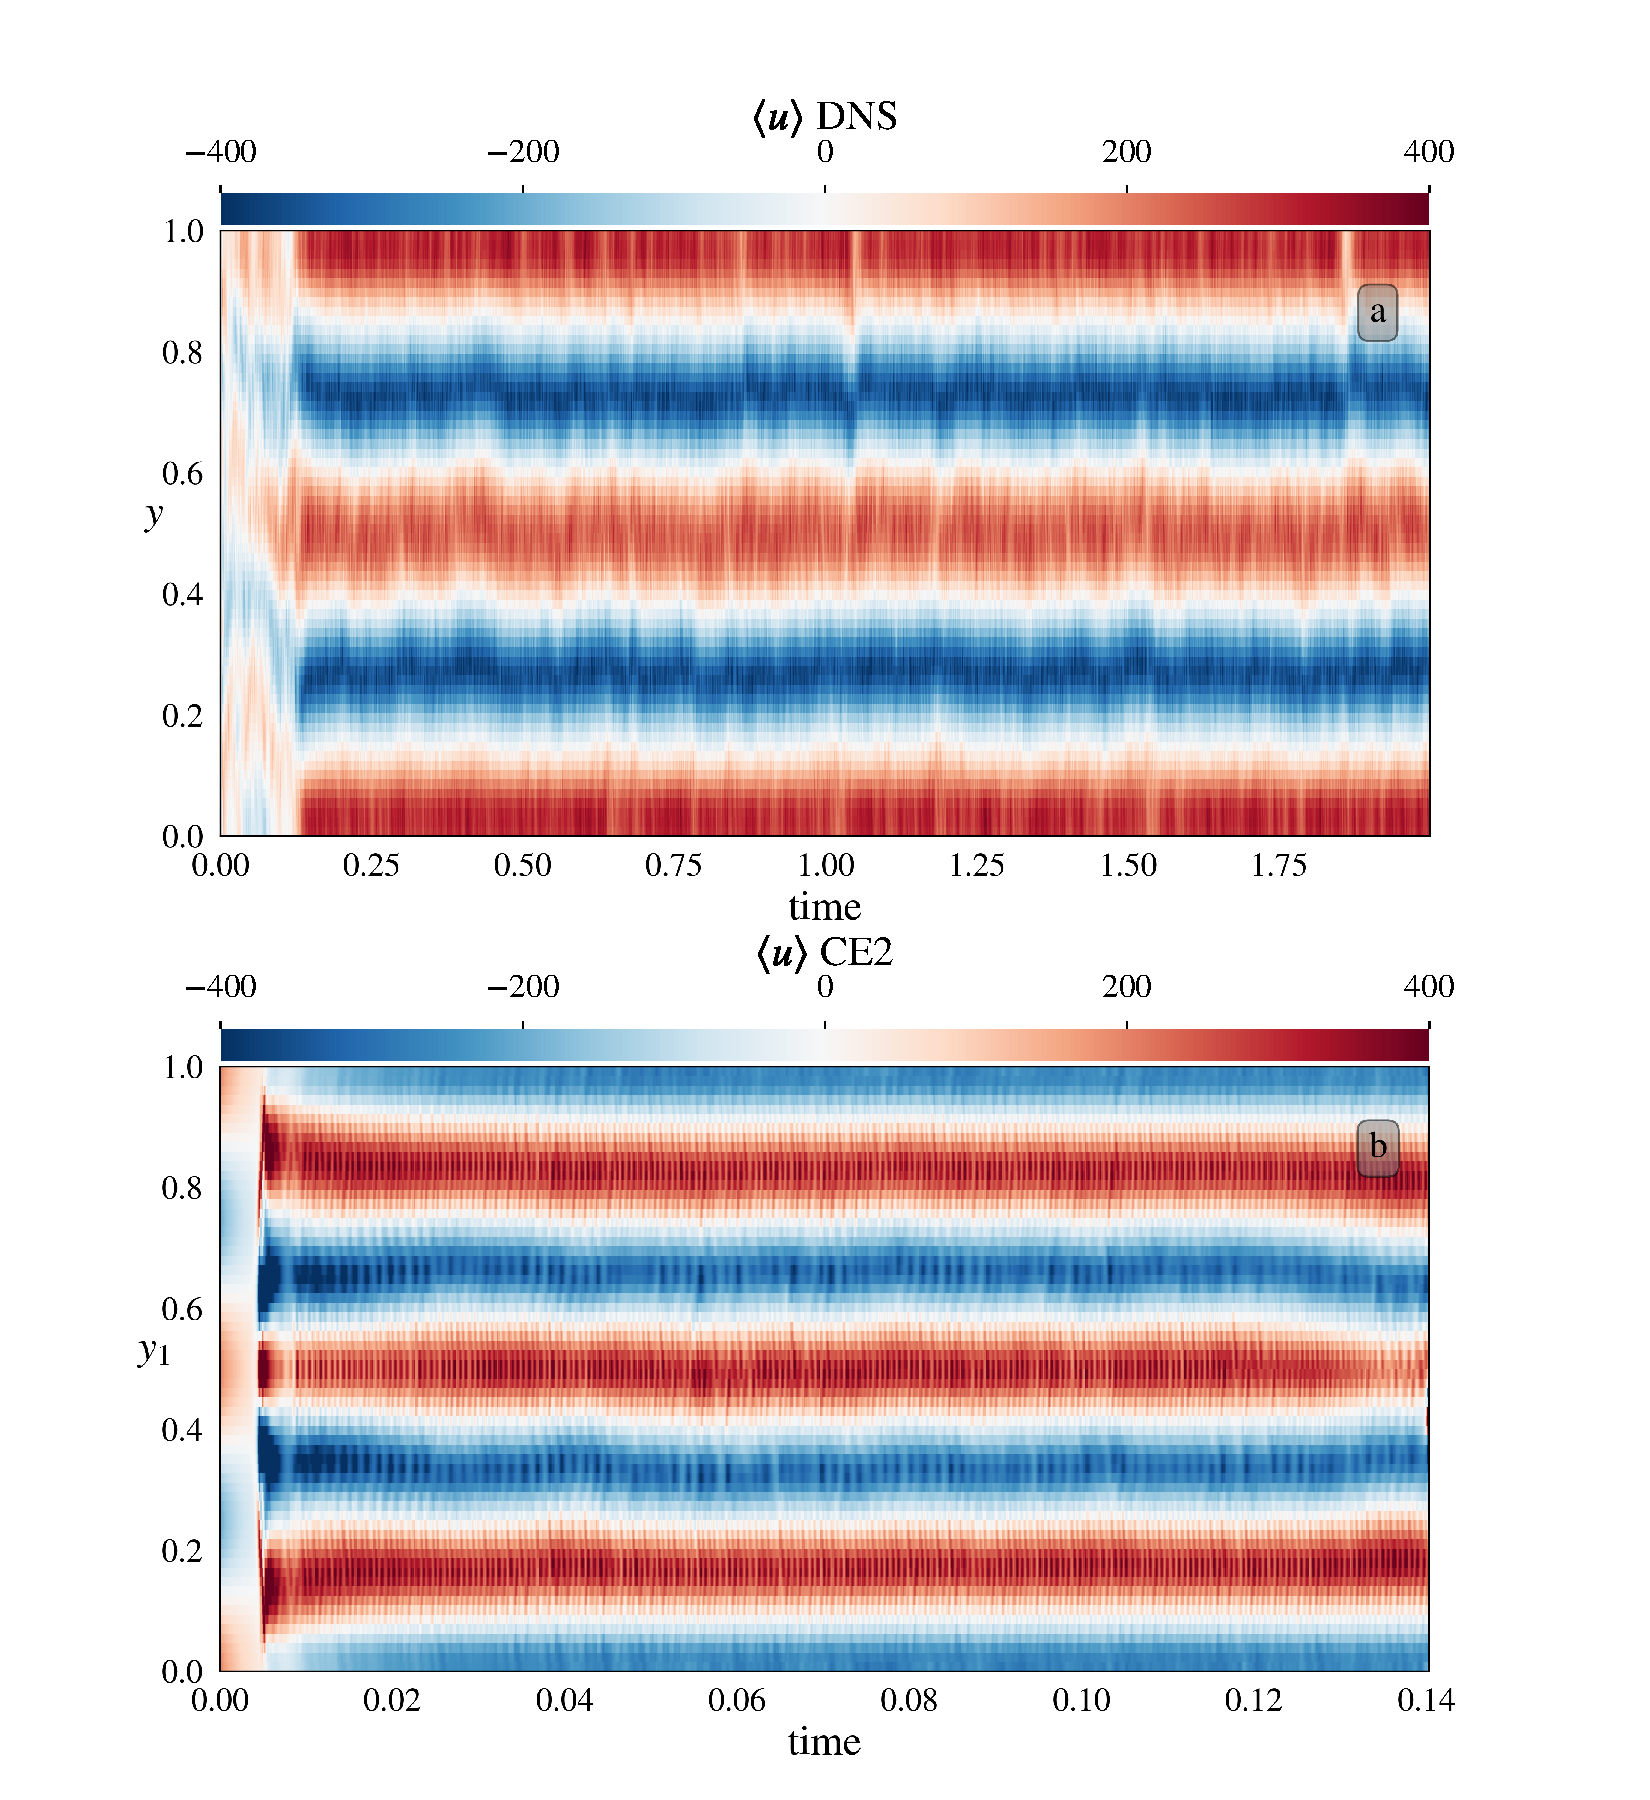
\includegraphics[width=0.5\textwidth]{../../figs/hov_cu_dns_ce2_run_T.pdf}
  \caption{Hovmoller diagram of run R in both DNS (a) and CE2 (b) with the CE2 solution biased with a 5-jet solution at $t=0$. Note that this picks up the incorrect 7-jet solution.}
  \label{fig:hov_run_T}
\end{figure}

\subsection{3 Jet to 2 Jet Transitions}
\label{sec:3->2}

In run A, the CE2 results return a 3-jet solution, while the DNS yields a 2-jet solution.
This is quite similar to the quasilinear run in \citet{2018RSPSA.47480422T}, which also produces a 3-jet solution.
Given that CE2 is fundamentally a quasi-linear theory, this is unsurprising.
However, a curious effect occurs in the DNS Hovmoller diagram:
the initial mean flow has three jets before a transition to a 2-jet solution occurs around $t \simeq X$.
One might hypothesize that the three jet solution and two jet solution coexist in the DNS but that the former has a faster growth rate but lower saturation amplitude than the latter.
In order to explore this idea, we biased the CE2 simulation by initializing the first cumulant of the x-velocity, $\cu$ to
\begin{equation}
  \label{eq:bias}
  \cu(t=0, y_0) = A_0 \left( \lambda cos(2\pi/L_y y_0) + (1-\lambda) cos (\pi/L_y y_0)\right).
\end{equation}
The first term is odd about the center of the domain, while the second is even\footnote{note that both have even parity with respect to the boundary connditions, as required by the boundary conditions}.
We use the linear boundary value solver in \emph{Dedalus} to solve for $c_\psi$ given $\cu$, and use this as an additional initial condition for $c_\psi$; in our unbiased simulations, $c_\psi(t=0) = 0$.
\begin{figure}
  \centering
  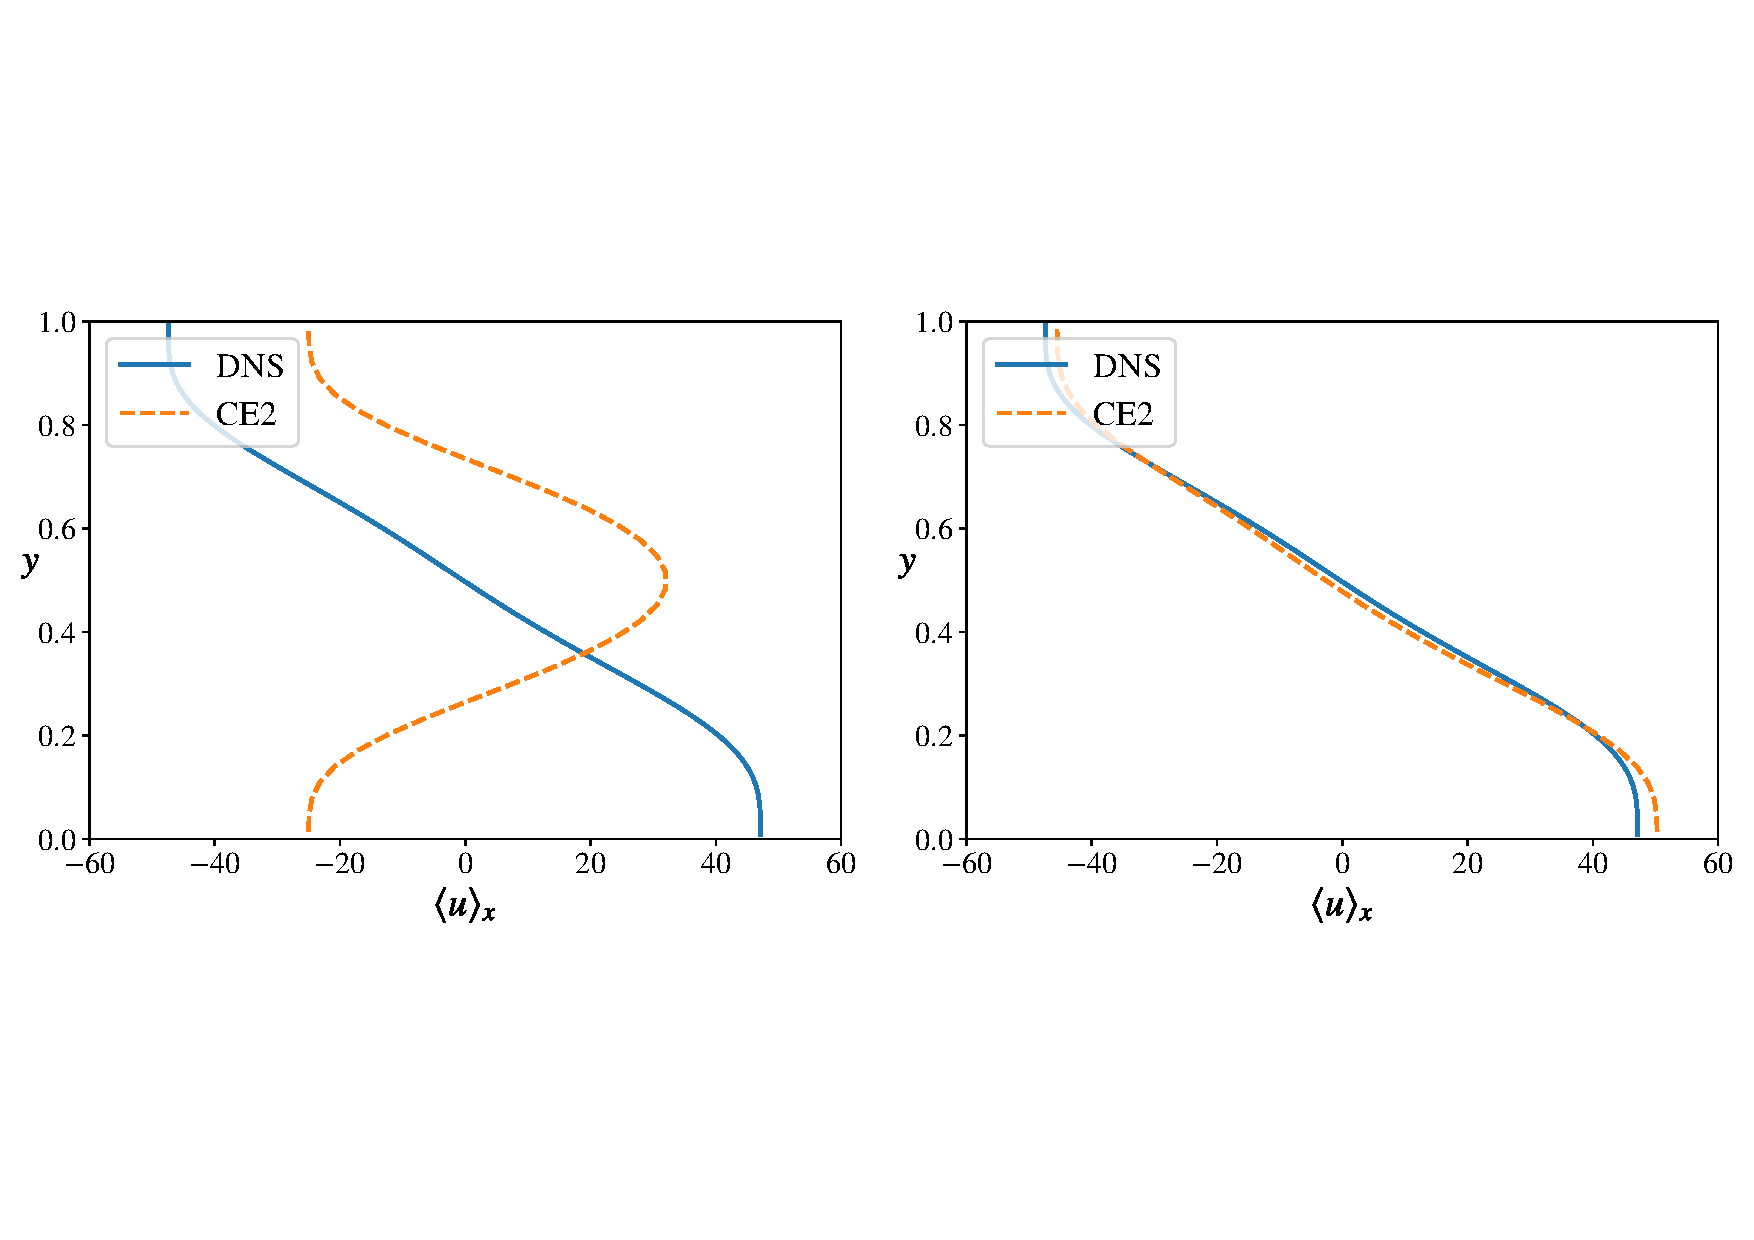
\includegraphics[width=\textwidth]{../../figs/umean_dns_ce2_runA_I.pdf}
  \caption{Time averaged $\cu$ as a function of $y$ for DNS (solid) and CE2 (dashed) for the run A parameters. On the left, the CE2 model was initialized with $\cu(t=0) = 0$; on the right $\cu(t=0)$ was set to a large-amplitude 2-jet solution.}
  \label{fig:cu_vs_y_runAI}
\end{figure}

\begin{figure}
  \centering
  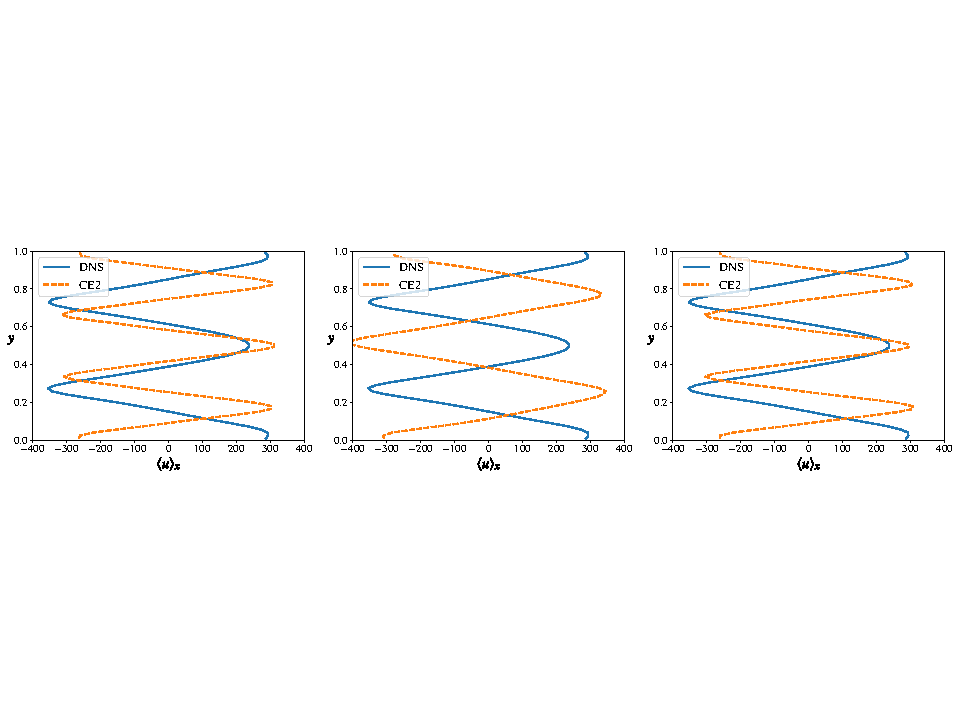
\includegraphics[width=\textwidth]{../../figs/umean_dns_ce2_runRST.pdf}
  \caption{Time averaged $\cu$ as a function of $y$ for DNS (solid) and CE2 (dashed) for the run R parameters. On the left, the CE2 model was initialized with $\cu(t=0) = 0$; in the middle $\cu(t=0)$ was set to a large-amplitude 3-jet solution; on the right $\cu(t=0)$ was set to a large-amplitude 5-jet solution. Oddly the 3-jet solution is the only one that finds the correct solution.}
  \label{fig:cu_vs_y_runRST}
\end{figure}

If the linear growth rate explanation is correct, then one would expect that for $\lambda \ll 1$ would lead the CE2 results to pick up the 2-jet solutions.
They do not.
However, CE2 \emph{is} capable of sustaining a 2-jet solution:
by biasing our simulation with $\lambda = 1$ and giving a substantial initial amplitude $A_0 = 40$, the CE2 results do reveal the 2-jet solution, and they saturate at an amplitude comparible to the DNS results.
This strongly suggests that the transition from 3 to 2 jets is the product of a subcritical, non-linear transition mediated by eddy-eddy $\to$ eddy interactions excluded from CE2 as well as our previous quasilinear results.
Regardless, this solution remains a fixed point of the CE2 system, suggesting that the \emph{selection} of a given multi-jet solution is distinct from its \emph{maintenence}.



% CE2 for bursting?
% What does CE2 get for 6 jet?

\subsection{Biasing higher jet counts}
\label{sec:higher_jet}


\subsection{Power Spectra}
\label{sec:powerspec}
Hi.
\begin{figure}
  \centering
  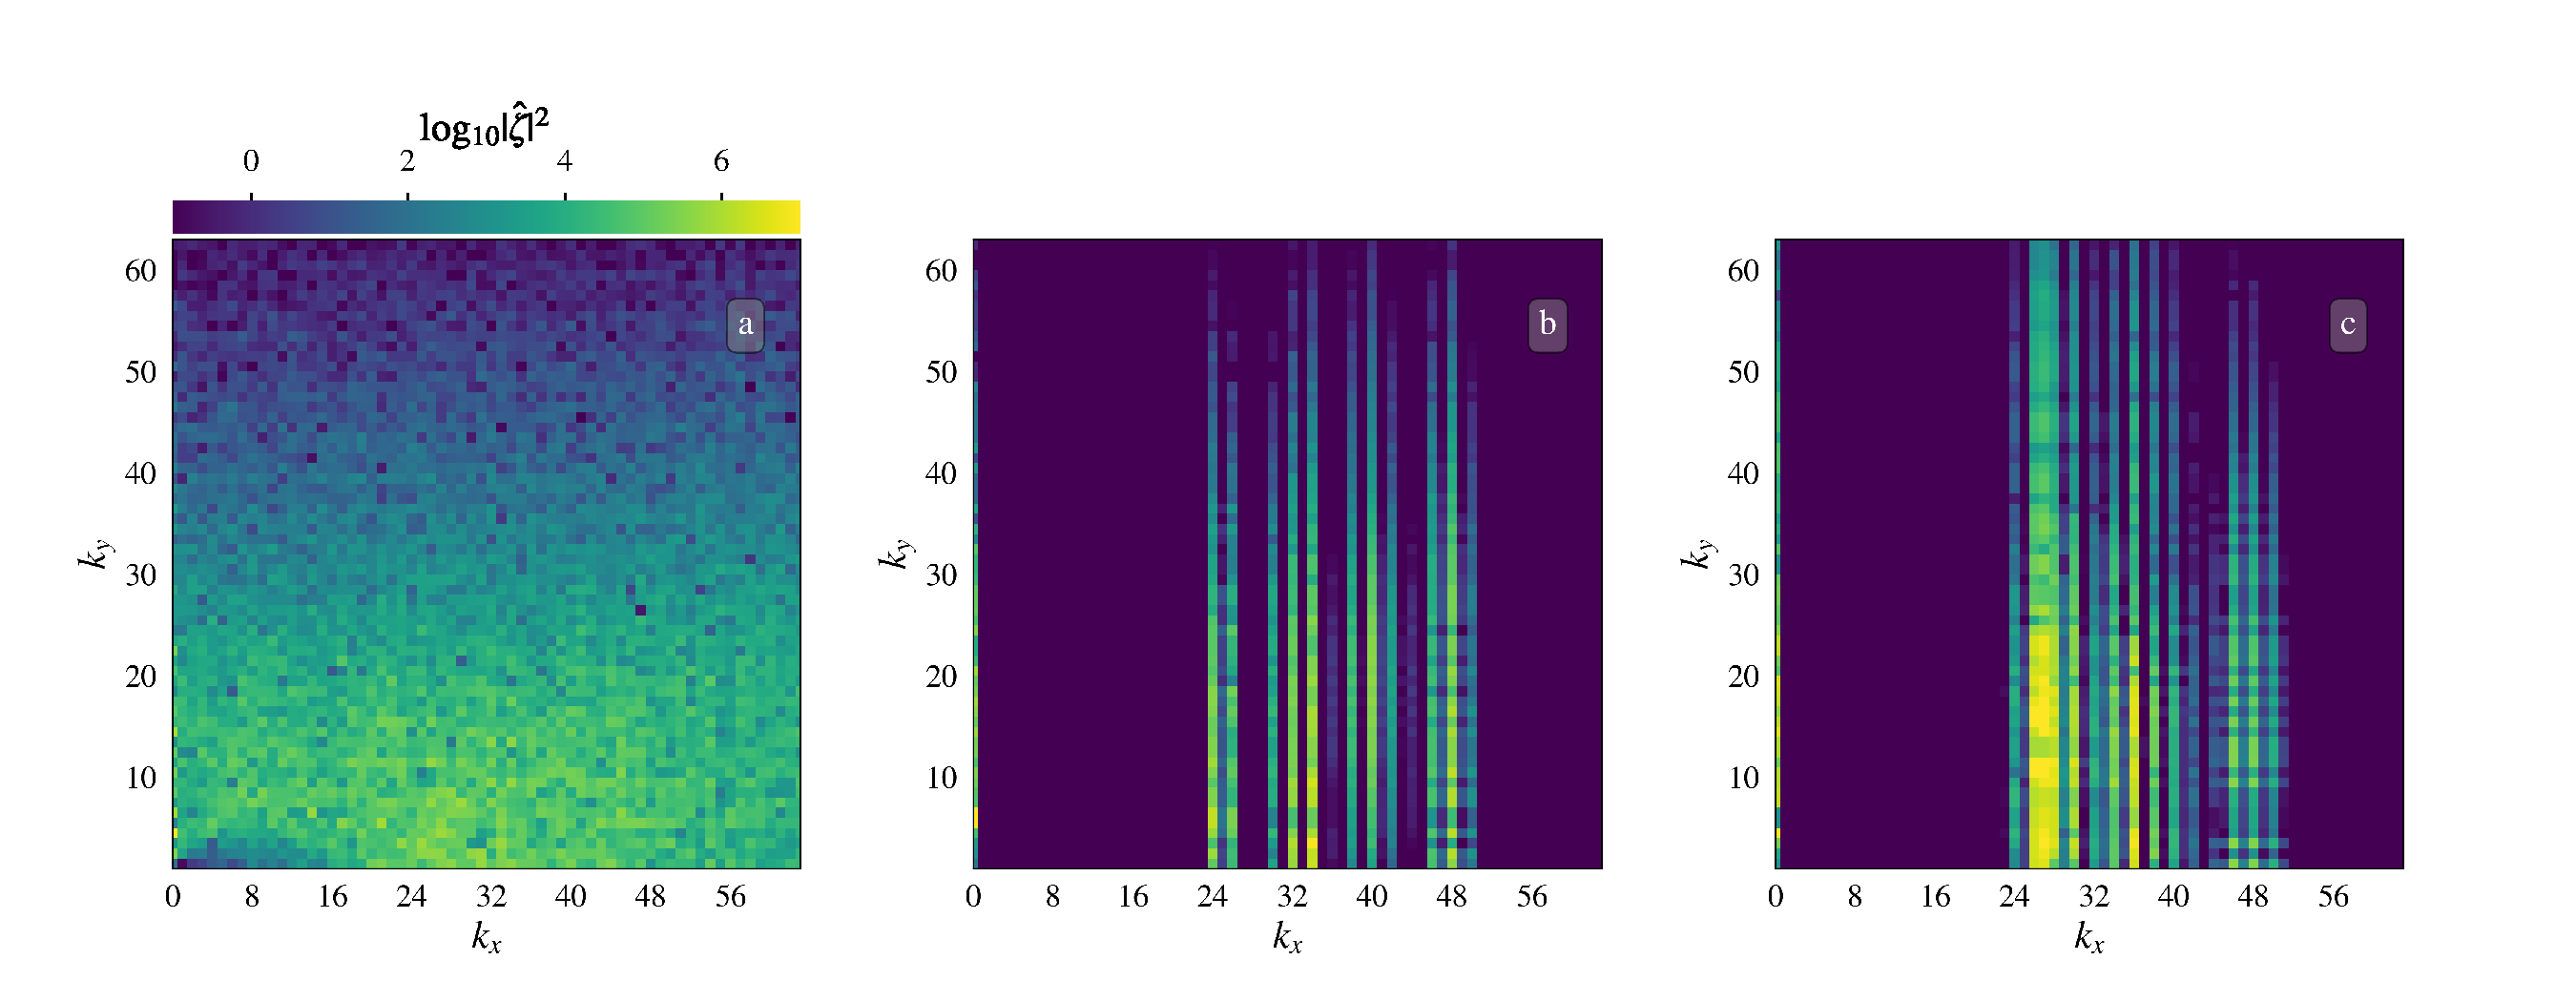
\includegraphics[width=\textwidth]{../../figs/power_spectra_zeta_dns_run_R.pdf}
  \caption{From left to right: power spectra of $\zeta$ from a) DNS, b) CE2 c) zonal ($k_x = 0$) spectra for run S.}
  \label{fig:power_spec_S}
\end{figure}


\subsection{PDFs}
\label{sec:pdf}

QL pdf vs NL pdf.
Does this do better than RB convection?

% \section{To Do}
% \label{sec:todo}

% \begin{todolist}
%   \item[\done] Fix drag runs
%     \begin{todolist}
%       \item[\done] restart a working run, adding small $C$. Does it crash?
%       \item[\done] run with each friction term off, one at a time
%     \end{todolist}
%   \item[\done] Look at 2nd cumulants
%   \item[\done] DNS with subtracted means: movie. Try to see if ``satellite modes'' are important. \textbf{Nope.}
%   \item plot DNS $k_x$ at a given height vs time.
%   \item Understand why QL/CE2 fail to reproduce correct number of jets. Is it that they can find all solutions, but cannot transition between them?
%   \item Project negative eigenvalues after run A without inline projection. Do we get the same solution? That is, are there multiple ICs that lead to similar results?
%   \item[\done] Power spectrum for $\psi$
%   \item[\done] Bias run R with 4-jet solution
%   \item[\done] Look at early time $t < 0.125$ in DNS run R. Is there a 7 jet solution present? 
%   \item Look at y-spectra for $k_x = 0$; try to see jet coalescence (maybe for paper 2) power timeseries like Bouchet et al PRL 2019?
%   \item[\done] Construct 2nd cumulants for DNS
%   \end{todolist}

\section{Fixed points and DNS to CE2 transitions}
\label{sec:fixed}
Statistical methods are most illuminating when we can probe their failures as well as their successes.
A key question is whether or not a steady-state solution of DNS is \emph{also} a steady-state of CE2.
In order to probe this, we computed the first and second cumulants from DNS data in three states: the steady, 2-jet solution at run A parameters, and representative burst and quiescent states from run C.

As expected from our prior experiment in which CE2 found the same solution as DNS when biased with a high-amplitude $\cu$ initial cindition, at run A parameters, CE2 is able to continue the DNS solution easily.
The 

\subsection{Run C}
\label{sec:run_c_dns_ce2}

Burst and quiet.

\section{Discussion}
\label{sec:discussion}

Emerging story: \emph{zonal} QL/CE2 fail to transition among states because they preclude $k_x = 1$ ``satellite'' modes. If we can restore the transition between states by going to \emph{ensemble} CE2, then this would give good evidence that that is the right approach.


Computations presented here were performed on the Bates High Performance Computing Center's \emph{Leavitt} system.
Computing Resources supporting this work were also provided by the NASA High-End Computing (HEC) Program through the NASA Advanced Supercomputing (NAS) Division at Ames Research Center with allocation GID s1647.
JSO was supported by NASA LWS grant No. NNX16AC92G, Research Corporation Scialog Collaborative Award (TDA) ID\#24231.


\appendix
\section{}\label{appA}
In order to ensure stability of the calculations at higher $\Rayleigh$, we have found it necessary to remove negative eigenvalues from the second cumulant at an interval of 10 timesteps.
While this is required for CE2.5 \citep{marston_qi_tobias_2019}, it appears necessary even in the CE2 simulations presented here.
The second cumulants must be positive definite in order to ensure the corresponding probability density function is realizable (that is, nowhere negative).


\bibliographystyle{jfm}
% Note the spaces between the initials
\bibliography{busse}

\end{document}

%  LocalWords:  DNS cumulants cumulant annulus
